\documentclass[11pt,a4paper]{article}
\usepackage[latin1]{inputenc}
\usepackage{amsmath}
\usepackage{amsfonts}
\usepackage{amssymb}
\usepackage{graphicx}
\usepackage{epstopdf}
\usepackage{color}
\usepackage[nottoc,notlot,notlof]{tocbibind}
\usepackage{float}

%code listings setting 
\usepackage{listings}
\definecolor{sapgreen}{rgb}{0.31, 0.49, 0.16}
\definecolor{royalazure}{rgb}{0.0, 0.22, 0.66}
\definecolor{rufous}{rgb}{0.66, 0.11, 0.03}
\lstset{
	breaklines=true,
    showstringspaces=false,
    language=Python,
    basicstyle=\ttfamily\footnotesize,
    commentstyle=\upshape\color{sapgreen},
    keywordstyle=\bfseries\color{royalazure},
    stringstyle=\color{rufous}
}

\author{Bartosz Animucki {\tt (1226153)} \\ Roman Kazus {\tt (1239966)}}
\title{2MMN40 Report: Modeling aqueous ethanol}

\begin{document}
\maketitle

\setcounter{secnumdepth}{2}
\setcounter{tocdepth}{2}
%\clearpage
\tableofcontents
\clearpage  
\section{Introduction}
Ever since ethyl alcohol was successfully distilled in high concentrations for the first time during the Islamic golden age \cite{first_distil}, (al)chemists and enthusiasts alike have been fascinated by its wide uses such as a medical and industrial solvent, as a substrate in organic chemistry, as a psychoactive substance, and many more. 
	
Nonetheless, perhaps the most important current research goal that involves the study of the properties of ethanol, especially in water mixtures, is biofuels \cite{quovadis} \cite{fuelcell}. Being derived from biomass sources, bio-ethanol contains water, no matter how efficiently it is distilled. This is because at about 95\% ethanol, the mixture is azeotropic -- meaning that neither ethanol nor water evaporate more when the mixture is heated. Further study of this phenomenon, as in \cite{azeobreak}, would be of immense value to the feasibility of biofuel production. 
	
The exact chemical properties of this type of water-ethanol mixtures, such as volume contraction, have also been studied extensively. One prominent theory of the origin of aqueous ethanol volume contraction, put forth by Frank and Evans \cite{frankevans}, hypothesized that water molecules form so-called ``icebergs'' around hydrophobic solute molecules. Under this theory, when ethanol molecules are introduced to water, the water molecules around the hydrophobic  end  of  the  ethanol  undergo  a  structural rearrangement in such a way that strong water-water hydrogen bonds are formed. This model was repeatedly tested and verified later on in prominent experimental studies such as \cite{parke}. Similar results were found in \cite{guoetal}.
	
In this report, we explore a basic computational model for predicting thermodynamic properties of water-ethanol mixtures using the principles of Molecular Dynamics.
	
\section{Theory}
\subsection{Molecular Dynamics}
\label{MD} % Don't delete this label
In the spirit of Molecular Dynamics, an ensemble of molecules is modeled with an application of classical mechanics. Newton's equations of motion are solved at each time step, with the forces calculated from a combination of bonded and non-bonded potentials. However, developing meaningful insights about thermodynamic properties of a particular chemical system requires many molecules to be included in the ensemble. This, together with the complexity of the physical interactions, makes it impractical (and often impossible) to solve such problems analytically. This is where computational simulations come in. \cite{wiki} We do have to notice that molecular modeling can be computationally challenging due to the number of chemical and physical interactions one needs to model. 

The system we consider can be described by a Hamiltonian system which describes the evolution equations of the physics occurring between the molecules. This means that the entire system is described at a given time by the positions $\mathbf{q}$ and momenta $\mathbf{p}$ of its particles. To describe the time evolution, we first define the Hamiltonian $\mathcal{H}\left( \mathbf{q}, \mathbf{p}, t \right)$. This quantity, denoted by $\mathcal{H}$ for short, describes the total energy of a closed system. In our case the total energy is given by the sum of the total kinetic energy and total potential energy of the particles in the system. In Appendix \ref{notation} we define some notation we use throughout this paper. We have for the energies:
\begin{align}
E_{kinetic} = \sum\limits_{i=1}^{N} \frac{||\textbf{p}_i||^2}{2\cdot m_i} \\
E_{potential} = V(\textbf{q})
\end{align}
where $V(\textbf{q})$ is a function to describe the potential energies of the atoms. In our case many interactions between atoms can be modeled by a potential function. Each interaction is seeking for a state in which it is in equilibrium, e.g. an O-H bond in water has a potential energy if they are not 0.9572 \AA $\;$ apart (bond potential) and a there is also an interaction between the 3 atoms H-O-H in water: it has a potential energy higher than the minimum if these are not in a $104.52^\circ$ angle (angle potential).

Between non-bonded atoms of different molecules (Van der Waals interactions) there is the so-called Lennard-Jones potential. In our case we model the potential energy as the sum of the bond potentials (between two bonded atoms), the angle potential (between three atoms making an angle with each other), the proper dihedral potential (between four atoms (chained in a row for proper dihedrals) making a planar angle with each other) and the Lennard-Jones (LJ) potential (between two atoms from different molecules). 

We restricted ourselves to the just mentioned potentials. Electrostatic potentials, many-body potentials and improper dihedral potentials are thus not included and are left for further research. 

Potential energy functions are often modeled by harmonic oscillators for the bond and angle potentials, by a periodic function (cosine form) for proper dihedrals and by the Lennard-Jones potential function for the Van der Waals interactions. Let $r_b$ be the distance between two atoms for bond $b$, let $\theta_a$ be the angle between the three atoms for angle $a$, let $\phi_{dih}$ be the torsion angle between four chained atoms for proper dihedral $dih$, let $\psi_{dih} = 180^\circ - \phi_{dih}$ and let $r_{LJ}$ be the distance between two atoms $i$ and $j$ which have a Van der Waals interaction. Then we have:

\begin{align*}
& V(\textbf{q}) & = & \; \; \; \sum\limits_{b\in all \; bonds}V_{bond}(r_b) +  \sum\limits_{b\in a;; \; bonds}V_{bond}(r_b) +  \sum\limits_{a\in all \; angles}V_{angle}(\theta_a) \\
& \textcolor{white}{.} & \textcolor{white}{.} & \; \; \; +  \sum\limits_{dih\in all \; prop. \; dih.}V_{dih.}(\psi_{dih}) + \sum\limits_{(i,j)\in all \; LJ-int.}V_{Lennard-Jones}(r_{ij}) \\
& V_{bond}(r) & = & \; \; \; \frac{1}{2}\kappa_{b}\left( r - r_0 \right)^2 \\
& V_{angle}(\theta) & = & \; \; \; \frac{1}{2}\kappa_{a}\left(\theta - \theta_0 \right)^2 \\
& V_{prop.\; dih.}(\psi) & = & \; \; \; \frac{1}{2}\left(C_1(1+\cos(\psi) + C_2(1-\cos(2\psi) + C_3(1+\cos(3\psi) + C_4(1-\cos(4\psi)) \right) \\
& V_{LJ}(r_{ij}) & = & \; \; \; 4\epsilon_{ij}\left(\frac{\sigma_{ij}^{12}}{r_{ij}^{12}} - \frac{\sigma_{ij}^{6}}{r_{ij}^{6}}\right)
\end{align*}
Note that $r$, $\theta$, $\psi$ and $r_{ij}$ can be well expressed in terms of the position $\textbf{q}$. These expression can be quite extensive and are omitted as we do not use them. Also note that all $\kappa_b$, $r_0$, $\theta_0$, $\kappa_{a}$, $C_1$, $C_2$, $C_3$, $C_4$, $\epsilon_{ij}$ and $\sigma_{ij}$ are all parameters of the model. 

We can now formulate our Hamiltonian:

\begin{align}
\mathcal{H}\left( \mathbf{q}, \mathbf{p}\right) = \sum\limits_{i=1}^{N} \frac{||\textbf{p}_i||^2}{2\cdot m_i} + V(\textbf{q})
\end{align}
From the potential energy we are able to calculate forces $F_i$ on atom $i$ as follows: $F_i = -\nabla_{\textbf{q}_i}V(\textbf{q})$. Of course Newton's second law must apply, so we get: $\nabla_{\textbf{q}_i}V(\textbf{q}) = -F_i = -m_i\ddot{\textbf{q}}_i$. Taking the Hamiltonian's gradient with respect to $\textbf{p}_i$ and to $\textbf{q}_i$ gives us the following:

\begin{align}
\nabla_{\textbf{p}_i} \mathcal{H}\left( \mathbf{q}, \mathbf{p}\right) = \frac{\textbf{p}_i}{m_i} = \frac{m_i \textrm{$\dot{\textbf{q}}$}_i}{m_i} = \textrm{$\dot{\textbf{q}}$}_i \\
\nabla_{\textbf{q}_i} \mathcal{H}\left( \mathbf{q}, \mathbf{p}\right) = \nabla_{\textbf{q}_i}V(\textbf{q}) = -F_i = -m_i\ddot{\textbf{q}}_i = -\dot{\textbf{p}}_i
\end{align}
These equation are called Hamilton's equations and form the evolution equations for our system:

\begin{align}
\frac{\mathrm{d}\textbf{q}}{\mathrm{d}t} &= \nabla_{\textbf{p}}\mathcal{H}\left( \mathbf{q}, \mathbf{p}\right)\\
\frac{\mathrm{d}\textbf{p}}{\mathrm{d}t} &= -\nabla_{\textbf{q}}\mathcal{H}\left( \mathbf{q}, \mathbf{p}\right)
\end{align}
Hamilton's equations together with an initial configuration of the system give an initial-value problem which can be integrated. This integration has to be done numerically since analytically there is no way to obtain the solution. Since the system suffers from Lyapunov instability, the systems behaves chaotically which makes analytical solutions even more challenging \cite{lyapunov}. When starting from the initial configuration and solving the Hamilton's equations numerically, we can choose our time domain as long as required.

We note that we model a so-called canonical ensemble, meaning that the number of molecules ($N$), volume ($V$), and temperature ($T$) are conserved. Another way of expressing this is that this is an \textit{NVT} ensemble. Conserving temperature is accomplished with a thermostat, discussed in a later section. Without this thermostat, the system would be microcanonical (\textit{NVE}), meaning that instead of temperature, energy (in the form of the Hamiltonian $\mathcal{H}$) is conserved over time. 

It should also be noted that in this microscopic context, temperature is defined in terms of average kinetic energy:

\begin{equation}
T = %\frac{2}{3 N  k_B} \left\langle \frac{p^2}{2m} \right\rangle = 
\frac{2}{3 k_B N} \left\langle \sum_{i=1}^N m_i \left\|\textbf{v}_i\right\|^2 \right\rangle, 
\end{equation}
where $k_B$ is the Boltzmann constant and where $\left\langle \cdot \right\rangle$ denotes the time average. This approach is valid, because in such a simulation, all atomic movements are known, and there is no need to take into account the rotational and vibrational degrees of freedom separately. These modes of motion are simply part of the motion that is included as part of the Hamiltonian formalism. 

Additionally, for inducing insights about large-scale systems from nano-scale molecular modeling, many analyses of simulations of this type assume the ergodic hypothesis. Ergodicity lets us replace phase space averages of thermodynamic parameters that result from the Hamiltonian with simpler averages over a trajectory, requiring fewer, smaller simulations \cite{oliveira2007ergodic}.

\subsection{Ethanol and water}

The mixing of ethanol and water is exothermic. This means that energy is released as heat when the substances are mixed. This has to do with hydrogen bonding; ethanol disrupts the strong hydrogen bonding qualities of pure water by introducing its own polarized O--H bond into the mix. Ethanol does not hydrogen bond as easily due to its larger size and the fact that it has only one polarized bond rather than the two present in water.

Classical MD can capture some of these electronic effects, however in this report we do not introduce the required potentials that would let us study them. Lennard-Jones, as parametrized here, does not reproduce hydrogen bonding very well. However, this model should be able to capture other properties, such as heat capacity, radial densities, and for more complicated molecules, hard problems such as protein folding and enzyme catalysis. It is nonetheless practical and important to test MD concepts on simpler molecules such as water and ethanol before using them to study proteins. 

\subsection{Integrator}

To illustrate the choice of integrator, we explore the difference between the Forward Euler method and Velocity Verlet. Explicit integration is used for ease of implementation. For this we simulate 1000 $H_2$ molecules using different integrators. We show the energy plots we obtained by using forward Euler and by using velocity Verlet as integrator in Figures \ref{fig:inteuler} and \ref{fig:intvv}. Perhaps the most striking feature of Figure \ref{fig:inteuler} is that total energy isn't constant. In fact, the energy drift is so extreme in this basic method that inducing any thermodynamic insights from this integrator would be entirely erroneous. In fact, this method amplifies undamped oscillations, which is the case in classical molecular motion.

Therefore, we turn to the symplectic (energy-preserving) family of integrators. One of the most well-studied members of this family is Velocity Verlet. It offers superior numerical stability to Forward Euler, a higher order of local error, and conserves energy at each integration step (Figure \ref{fig:intvv}). We formulate the used velocity Verlet algorithm here:

\begin{align*}
\textbf{q}_i(t+\Delta t) &= \textbf{q}_i(t) + \Delta \textbf{v}(t) + \frac{(\Delta t)^2}{2m_i}\textbf{F}_i(\textbf{q}(t)) \\
\textbf{v}_i(t+\Delta t) &= \textbf{v}_i(t) + \frac{\Delta t}{2m_i}\left(\textbf{F}_i(\textbf{q}(t))+\textbf{F}_i(\textbf{q}(t+\Delta t))\right)
\end{align*}

\section{Simulation}
\subsection{Systems}
\label{system}
In this paper we study the molecular dynamics of ethanol mixtures. For that reason we consider three different systems:
\begin{itemize}
\item A system of pure water
\item A system of pure ethanol
\item A system of 13.5\% v/v ethanol in water
\end{itemize}
These systems are simulated at 300 Kelvin. In order to obtain a good picture on what happens over time in our system, we simulate for a period of 0.1 ns = 100000 fs. We take 2 fs as a timestep. Since computation effort increase rapidly with the number of molecules in the system, we can only simulate about 1000 molecules for 0.1 ns due to time and computational power constraints. From the density of water, the molecular weight and Avogadro's number, we can calculate that about 1000 molecules of water fit in a box of $31 \text{\AA} \times 31 \text{\AA} \times 31 \text{\AA}$. Therefore we take a box size of 31 \AA. Analogously, for pure ethanol, 308 molecules fit in this box. For 13.5\% ethanol in water, 906 molecules fit in the box.   

\subsection{Forces}
The given bonded, angle, dihedral potential and Lennard-Jones potential require parameters which depend on the atoms and molecules. For the purposes of this report, we used parameters derived from the TIP3P water model \cite{tip3p} and OPLS/AA all-atom carbohydrate force field \cite{oplsaa}. \\The potentials given in section \ref{MD} cause forces on the atoms. We find the force on an atom $i$ by taking minus the gradient of the potential with respect to $\textbf{q}_i$. Often, the potential is not expressed in terms of $\textbf{q}_i$ and this expression is often mathematically very extensive. Fortunately, we do not need to express these functions in $\textbf{q}_i$ explicitly as we can make use of the chain rule or of some geometric properties.

For the bond potential, we clearly know the direction of the force: attractive if $r > r_0$ (pointing towards the interacting atom) and repulsive if $r < r_0$ (pointing away from the interacting atom). The magnitude is readily found by the chain rule:    
%For the bond potential between bonded atoms $i$ and $j$ we get:

\begin{align*}
||F_i|| = \left\|-\nabla_{\textbf{q}_i}V(r)\right\| = \left\|\frac{\partial V}{\partial r}\right\| \cdot \left\|\nabla_{\textbf{q}_i}r\right\| = \kappa_{b}| r - r_0 |\frac{||\textbf{q}_i - \textbf{q}_j||}{r} = \kappa_{b}| r - r_0 |
\end{align*}
For the angle potential for the angle from atom $i$ via $j$ to $k$ with angle $\theta_{ijk}$, we know that the force's direction is orthogonal to the bond $ij$ and $jk$ and point inwards if $\theta > \theta_0$ and outwards if $\theta < \theta_0$. We use cross products to find these directions. The force on atom $j$ is minus the sum of the forces on atoms $i$ and $k$ since the sum of all forces need to be zero by Newton's first law. The magnitudes of the forces on atom $i$ and atom $k$ are given here:

\begin{align*}
\left\|F_i\right\| = \left\|-\nabla_{\textbf{q}_i}V(\theta)\right\| = \left\|\frac{\partial V}{\partial \theta}\right\| \cdot \left\|\nabla_{\textbf{q}_i}\theta\right\| = \kappa_{a}| \theta - \theta_0 | \frac{1}{||\textbf{q}_i - \textbf{q}_j||}= \kappa_{\theta}\frac{| \theta - \theta_0 |}{r_{ij}} 
\end{align*}
\begin{align*}
\left\|F_k\right\| = \kappa_{\theta}\frac{| \theta - \theta_0 |}{r_{kj}}
\end{align*}
For the proper dihedral potential for the dihedral from atom $i$ via $j$ via $k$ to $l$ with torsion angle $\theta_{ijkl}$ and $\psi_{ijkl}= \theta_{ijkl} - 180^{\circ}$, we follow the paper by Monasse and Boussinot \cite{hal} which gives derivations of the forces for each atom in the dihedral structure by using the fact that Newton's first law has to hold (the sum of forces is zero) and that the torque has to be zero as well (so we avoid rotation). We refer to the just mentioned paper for the derivations as they are straightforward but cumbersome.

For the Lennard-Jones potential for Van der Waals interactions between atom $i$ and atom $j$ which are not in the same molecule, we know that the atom's forces are attractive if $r_{ij} > \sqrt[6]{2}\sigma_{ij}$ and repulsive if $r_{ij} < \sqrt[6]{2}\sigma_{ij}$. Due to the boundary conditions of our system we do have to be careful when calculating the direction of the forces as we will explain later in section \ref{pbc}. The magnitude of the force is readily computed:

\begin{align*}
||F_i|| &= \left\|-\nabla_{\textbf{q}_i}V(r_{ij})\right\| = \left\|-\frac{\partial V}{\partial r}\nabla_{\textbf{q}_i}r\right\| \\
&= \left\|4\epsilon_{ij}\left(12\sigma_{ij}^{12}r_{ij}^{-13} - 6\sigma_{ij}^{6}r_{ij}^{-7}\right)\right\|\cdot \frac{||\textbf{q}_i - \textbf{q}_j||}{r} \\
&= 24\epsilon_{ij}\left|2\sigma_{ij}^{12}r_{ij}^{-13} - \sigma_{ij}^{6}r_{ij}^{-7}\right|
\end{align*}
To obtain the parameters $\epsilon_{ij}$ and $\sigma_{ij}$ we use so-called Lorentz-Berthelot mixing rules \cite{delhommelle2001inadequacy}:
\begin{align*}
\sigma_{ij} = \frac{1}{2}\left(\sigma_i + \sigma_j\right) \\
\epsilon_{ij} = \sqrt[]{\epsilon_i \epsilon_j}
\end{align*}
In order to reduce the computation effort, a Lennard-Jones cut-off distance is used. Since the Lennard-Jones potential is virtually zero for $r_{ij} > 8$ \r{A}, we do not calculate Van der Waals interactions if the distance between two atoms is more than 8 \r{A}. Also when $\epsilon_{ij} = 0$ or $\sigma_{ij} = 0$, we do not need to consider the Van der Waals interaction. These reductions of calculation speed up our simulation code immensely. 

The computational forms of our force calculations were successfully verified against \cite{hal}, so we are reasonably confident of their correctness.


\subsection{Periodic boundary conditions}
\label{pbc} % Don't delete this label due to a reference. 
As simulating molecular dynamics is very expensive in terms of computational effort, we cannot simulate even the tiniest part of a droplet of water as so many molecules are involved. Therefore, we must find other ways to simulate large amounts of molecules. This is usually done by defining periodic boundary conditions in our box of $x$ molecules ($x \approx 1000$, see section \ref{system}) which means that molecules move out at one side of the box, move in on the other side. Also, atoms can interact with other atoms on the other side of the box due to the fact that they are actually very close to each other when taking the periodicity of the boundary condition into account. If one would paste the same box with the same molecules on all sides of the box one could observe which molecules are close to each other (although they seem to be on the other side of the box). The periodic boundary conditions are visualized in Figure \ref{fig:pbc}.

In our implementation we let the molecules travel freely through space. We can then put them back into our box by applying the modulo operation (mod 'box size') on the $x$, $y$ and $z$ coordinates so that those are mapped back into the box. When considering bond, angle or dihedral potentials, we do not need to take into account more than the interactions within a molecule so we can calculate this in free space. However, when considering the Van der Waals interactions with the Lennard-Jones potential, we do have to take into account the boundaries. Let us take the box size of $31\text{\AA} \times 31\text{\AA} \times 31\text{\AA}$. If molecule $i$ is at $(x, y, z)_i = (61, -29, 1)$ and atom $j$ is at $(x, y, z)_j = (-28, 87, 32)$, the Lennard-Jones distances between these molecules is definitely not $((61-(-28))^2+(-29-87)^2+(1-32)^2)^{\frac{1}{2}} = 149.46$. To calculate this distance we have to keep subtracting or adding 31 from each coordinate until it is in the range [0, 31]. We thus get: $(x, y, z)_i = (30, 2, 1)$ and atom $j$ is at $(x, y, z)_j = (3, 25, 1)$. We then consider the difference between the coordinates: $(r_x, r_y, r_z) = (|30-3|, |2-25|, |1-1|) = (27, 23, 0)$. Since $r_x, r_y > \frac{1}{2}\cdot 31$, it is shorter to go from atom $i$ and atom $j$ through the $x$ and $y$ boundaries so that the distances are only $(|27-31|, |23-31|, 0) = (4, 8, 0)$ which gives $r_{ij} = (4^2 + 8^2 + 0^2)^{\frac{1}{2}} = 8.94$. This approach is mathematically translated to the following:
\begin{align*}
r_x &= |q_{ix} - q_{jx}| \\
r_y &= |q_{iy} - q_{jy}| \\
r_z &= |q_{iz} - q_{jz}| \\
r_x^* &= r_x - \text{boxsize}\cdot \left \lfloor{\frac{r_x}{\text{boxsize}}+\frac{1}{2}}\right \rfloor \\
r_y^* &= r_y - \text{boxsize}\cdot \left \lfloor{\frac{r_y}{\text{boxsize}}+\frac{1}{2}}\right \rfloor \\
r_z^* &= r_z - \text{boxsize}\cdot \left \lfloor{\frac{r_z}{\text{boxsize}}+\frac{1}{2}}\right \rfloor \\
r_{ij} &= \sqrt[]{r_x^{*2}+r_y^{*2}+r_z^{*2}}
\end{align*}

This distance $r_{ij}$ is used for calculations of the Lennard-Jones potential. The resulting force is either attractive (when $r_{ij} > \sqrt[6]{2}\sigma_{ij}$) or repulsive (when $r_{ij} < \sqrt[6]{2}\sigma_{ij}$). The direction of the force is the direction over which the distance $r_{ij}$ is obtained. This calculation involves the same structure as mentioned above. 

\subsection{Thermostat}
In order to keep the temperature at 300 Kelvin during our simulations, we have to make use of a thermostat. If one does not use a thermostat which keeps the temperature constant, the potential energies in the system may cause the molecules to rapidly increase their kinetic energy by which the temperature rises. When temperature is not hold constant, one cannot study the physical and chemical properties of a system well as these may change because of temperature fluctuations. Also, when doing simulations, the kinetic and potential energies might reinforce each other and due to the discreteness of numerical integration, velocities could explode and let molecules collide.

As we mentioned in section \ref{MD}, the temperature of the system is given in terms of the time average of the total kinetic energy of all atoms scaled with some constant. A very naive but straightforward and computationally inexpensive way to keep the temperature constant is by rescaling the momenta (or velocities) in the system every time the temperature deviates from our target temperature of 300 Kelvin. Experimentally this would be done by using a temperature regulating laboratory bath where temperature can be regulated. In our simulations we rescaled our momenta in the following way:  
\begin{align*}
\textbf{p}_{new} = \sqrt[]{\frac{300}{T}}\textbf{p}_{old}
\end{align*}
where $\textbf{p}_{old}$ is the momentum vector before rescaling and $T = \frac{2}{3 k_B N} \left\langle \sum_{i=1}^N \frac{\left\|\textbf{p}_i\right\|^2}{m_i}\right\rangle$. The time average is only taken over one period since we really want no fluctuations in temperature. In experiments this is often impossible to achieve but in simulations this is which is an advantage of simulations making it possible to study our mixture in a more theoretical way. 

\subsection{Code structure}
The code we used to simulate our systems is given in appendix \ref{code}. The code has 12 parameters which the user can define: the integrator which is to be used (Euler, Verlet or velocity Verlet), the timestep for numerical integration (in fs), the total time of the simulation (in fs), the box size (one side of the cube, in \AA), the total number of molecules, the percentage of ethanol (in \%), a parameter which determines whether we rescale momenta each timestep (thermostat), the target temperature for the thermostat (in K), the file name to write the output to, the Lennard-Jones cut-off distance (in \AA), the mean of the initial velocities and the standard deviation of the initial velocities. The structure of the code is summarized as a flowchart in Figure \ref{fig:flowchart}.

Our initial configuration of the system is made by putting the number of molecules in a three-dimensional square grid and giving the molecules normally distributed velocity components. 

\section{Results and discussion}

\subsection{Energies and temperature}

The energy profiles of the three simulations are shown in Figures \ref{fig:ewater1}-\ref{fig:emix2} at two different timescales. At short timescales, the simulation shows very jagged energy oscillations; this has to do with the fact that energy oscillates with twice the frequency of velocity oscillations. In the O--H bonds, the spring constant $k/N_A$ is on the order of $500000 \text{ kJ}\text{ mol}^{-1}\text{ nm}^{-2}$. Given that the reduced mass $\mu$ is no more than the mass of the hydrogen, we can quickly estimate that the smallest period of oscillation we expect is no larger than roughly

\begin{equation}
2 \pi \sqrt{\frac{\mu}{k}} \leq 2 \pi \sqrt{\frac{1\text{ u}}{500000 \text{ kJ}\text{ mol}^{-1}\text{ nm}^{-2} \cdot N_A}} \approx 8.9\text{ fs}.
\end{equation}
Since we are required to use an integration step of 2 fs, this oscillation gets close to causing numerical instability. It would be prudent to use shorter timesteps than 2 fs for this reason. This would unfortunately make simulation much more expensive computationally. 

The kinetic energy is held constant by the thermostat, which in turn causes the total energy to fluctuate. In the long-term figures (\ref{fig:ewater2}, \ref{fig:eethanol2}, \ref{fig:emix2}), it is evident that over the longer course of the simulation this energy does eventually settle around an equilibrium zone. 

The code constantly measures temperature, and adjusts it to the required level, as evidenced by the constant sum of kinetic energy in the ensemble. 

\subsection{Radial distribution functions}

The water profiles (Figure \ref{fig:rdfwater}) match up to the radial distribution functions in literature \cite{radial} in the close neighborhood of the reference particle. However, beyond about 7\AA, the distortion is caused by the fact that the molecules are in a microscopic box, rather than a large body of liquid. In a future iteration, the RDF calculation code could be improved to take the periodic boundary conditions into account, and average the distances over time.

In simulations that included ethanol, the total number of molecules was much smaller, leading to very poor and noisy estimations of the radial density functions (Figures \ref{fig:rdfethanol} and \ref{fig:rdfmix}).

\subsection{What can be improved}
Although molecular modeling is known to be computationally very expensive and time consuming, we believe that our code could be optimized in several aspects. One of these is to get rid of the for-loops in our code as for-loops are very slow in Python when the number of iterations is high (e.g. for Lennard-Jones calculations). The for-loops in our 'calculateForcesEnergy'-function can be avoid rather easily by vectorization. We believe that the for-loop to do the numerical integration is more difficult to get rid of. If it were possible, we would have memory problems because our XYZ vector would become too large. Also, the many 'if'-statements could be drastically reduced to increase efficiency in our code. \\
In terms of computation power, one could investigate whether some computations could be done in parallel on several machines. We believe that the force calculation could really well be parallelized. \\
Our initialization of the positions could well be improved by defining another grid in order to allow any number of molecules instead of restriction that it has to be a power of three as it is now. Also, the square grid does not very well capture how it is in reality. However, the initial random velocities make the system chaotic (as in reality) really soon. \\
Physically speaking, one would want to incorporate forces caused by electrostatic potentials as well in order to capture the real physics in the system even more. Implementing this is not hard at all as the Coulomb potential is commonly used for this and is easy to implement and calculate. However, the number of Coulomb interactions gets quite large with the number of molecules in the system as with the Lennard-Jones potential, so vectorization is a must here as well to avoid too high computation costs. \\
\\ If all these improvements would be implemented, the code would be able to simulate much faster and closer to reality. However, we need to keep in mind that it is still a simulation and that molecular simulations are incredibly expensive in terms of computational cost.


\section{Conclusion}
In this report, we explored a basic computational model for predicting thermodynamic properties of water, ethanol, and water-ethanol mixture using the principles of Molecular Dynamics. 

We saw that there are many theoretical and programmatic challenges in the way of full, generalized implementations of Molecular Dynamics. However, even with a simple application of the basic theories, some chemical properties, such as radial distributions, can be matched to analytic solutions and experimental data. With focused research and development, these principles can be expanded to all sorts of molecular systems.


\clearpage
\bibliography{bibliography}
\bibliographystyle{alpha}

\clearpage
\appendix
\section{Figures}

\begin{figure}[ht]
\centering
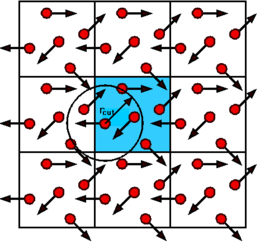
\includegraphics[scale=0.6]{figures/PeriodicBoundaryConditions}
\caption{Periodic boundary conditions visualized}\label{fig:pbc}
\end{figure}

\begin{figure}
\centering
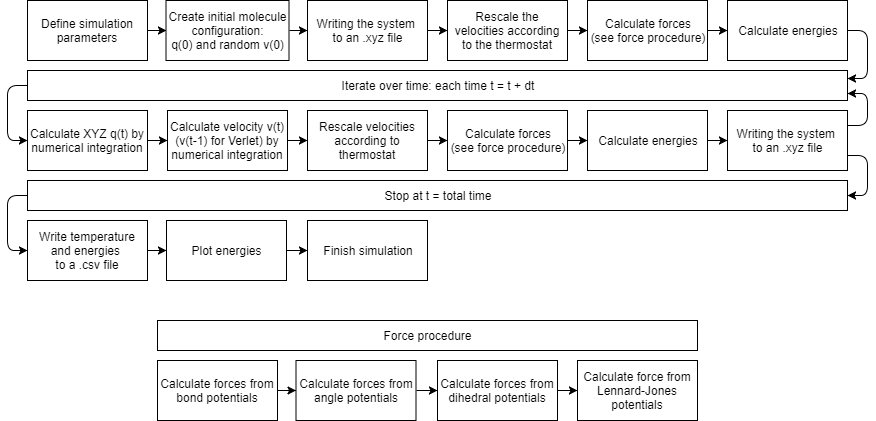
\includegraphics[scale=0.45]{FlowChartMD.png}
\caption{Code flowchart}\label{fig:flowchart}
\end{figure} 

\begin{figure}
\centering
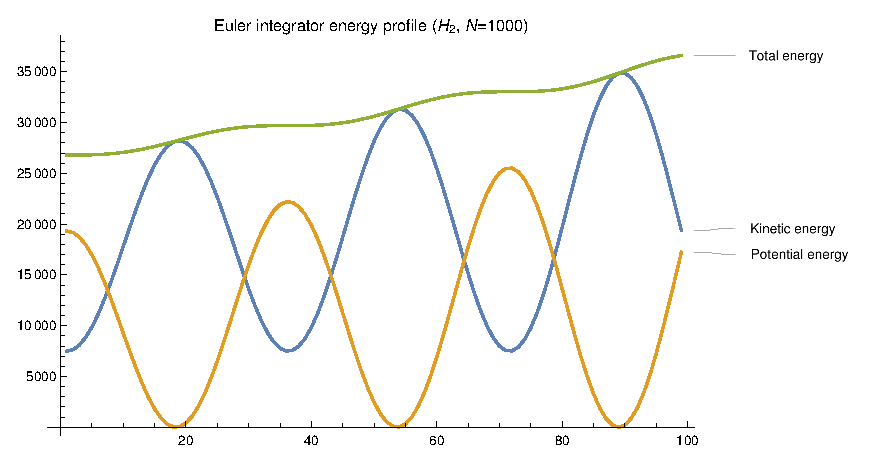
\includegraphics[scale=0.8]{figures/inteuler}
\caption{Energy profile for a 100-step run of the Forward Euler method in 1000 hydrogen molecules in a $\left(265\text{\AA}\right)^3$ box.}\label{fig:inteuler}
\end{figure}

\begin{figure}
\centering
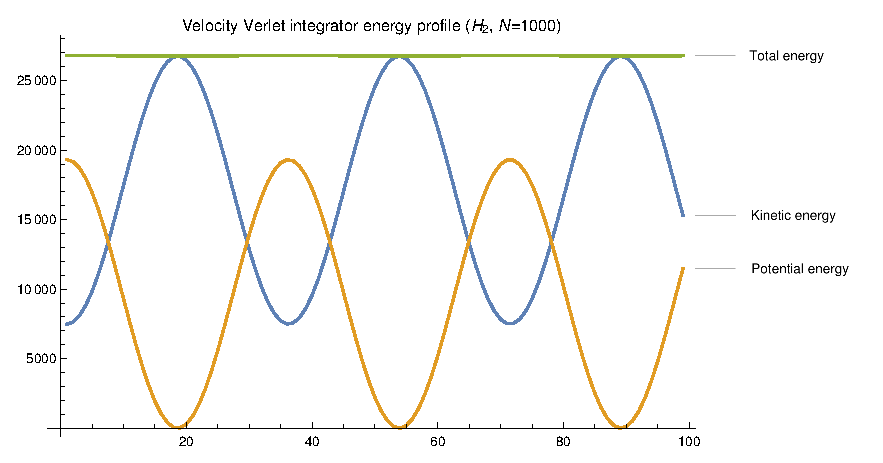
\includegraphics[scale=0.8]{figures/intvv}
\caption{Energy profile for a 100-step run of Velocity Verlet in 1000 hydrogen molecules in a $\left(265\text{\AA}\right)^3$ box.}\label{fig:intvv}
\end{figure}

\begin{figure}
\centering
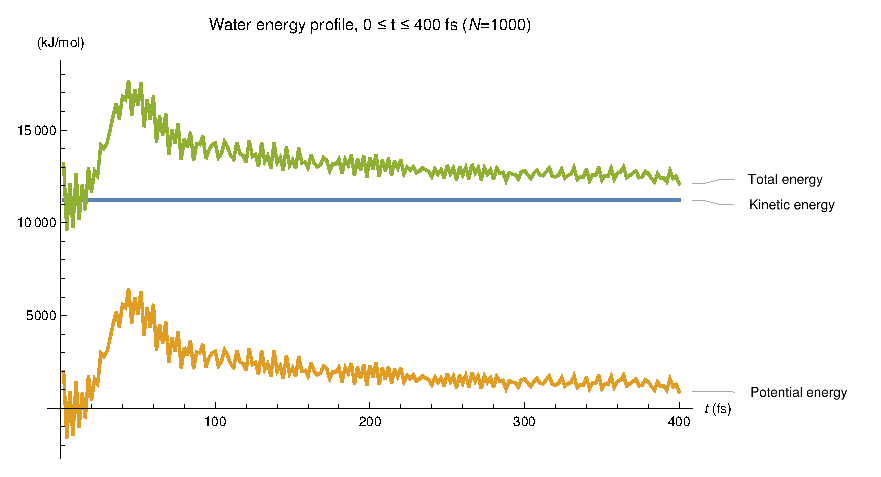
\includegraphics[scale=0.8]{figures/ewater1}
\caption{Energy profile of pure water simulation at 300K - first steps}\label{fig:ewater1}
\end{figure}

\begin{figure}
\centering
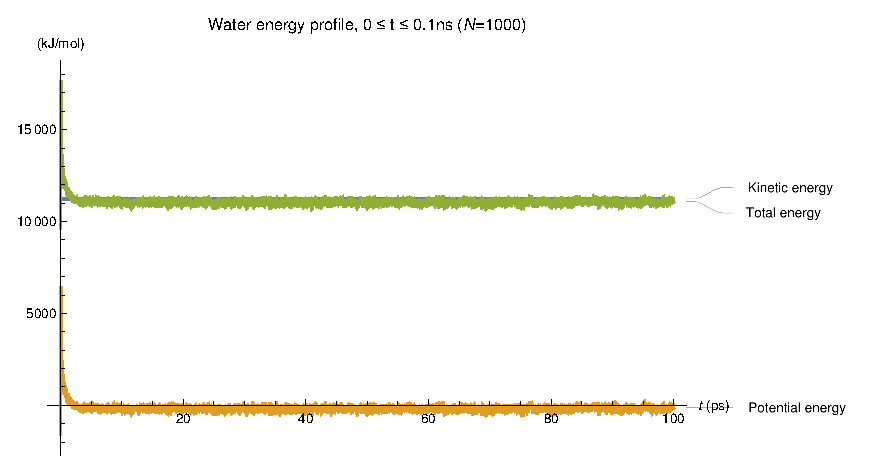
\includegraphics[scale=0.8]{figures/ewater2}
\caption{Energy profile of pure water simulation at 300K - complete}\label{fig:ewater2}
\end{figure}

\begin{figure}
\centering
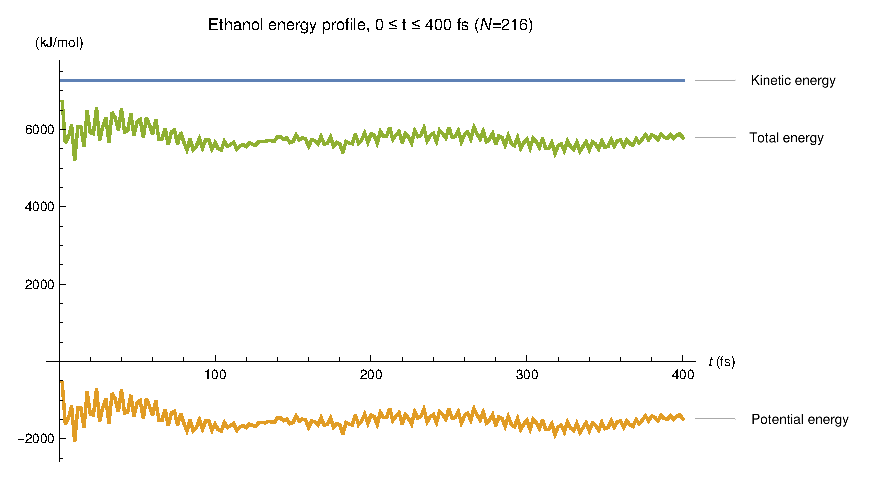
\includegraphics[scale=0.8]{figures/eethanol1}
\caption{Energy profile of pure ethanol simulation at 300K - first steps}\label{fig:eethanol1}
\end{figure}


\begin{figure}
\centering
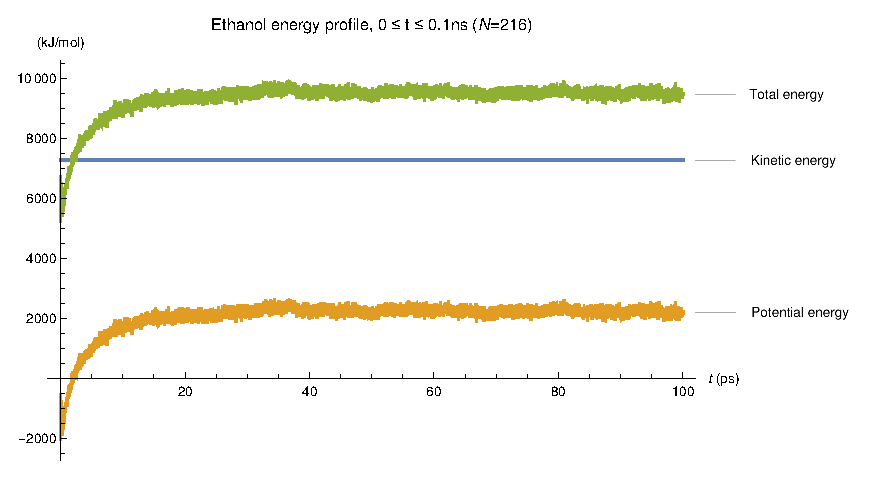
\includegraphics[scale=0.8]{figures/eethanol2}
\caption{Energy profile of pure ethanol simulation at 300K - complete}\label{fig:eethanol2}
\end{figure}

\begin{figure}
\centering
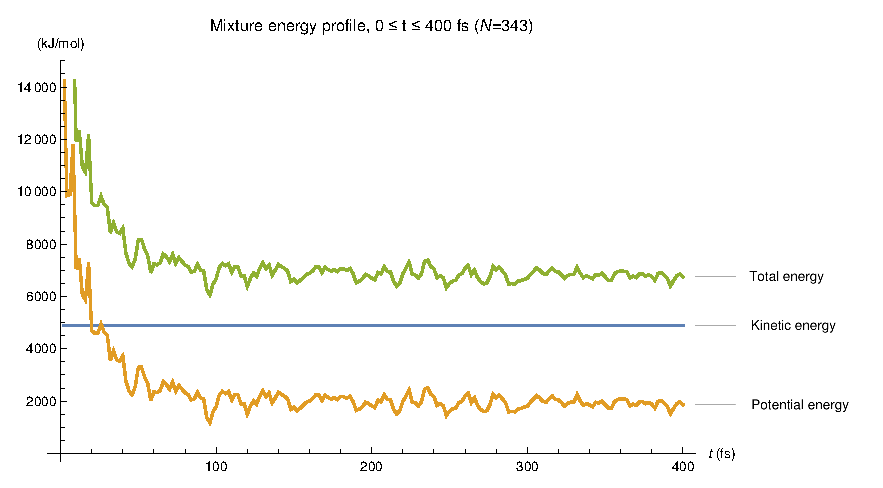
\includegraphics[scale=0.8]{figures/emix1}
\caption{Energy profile of 13.5\% mixture simulation at 300K - first steps}\label{fig:emix1}
\end{figure}

\begin{figure}
\centering
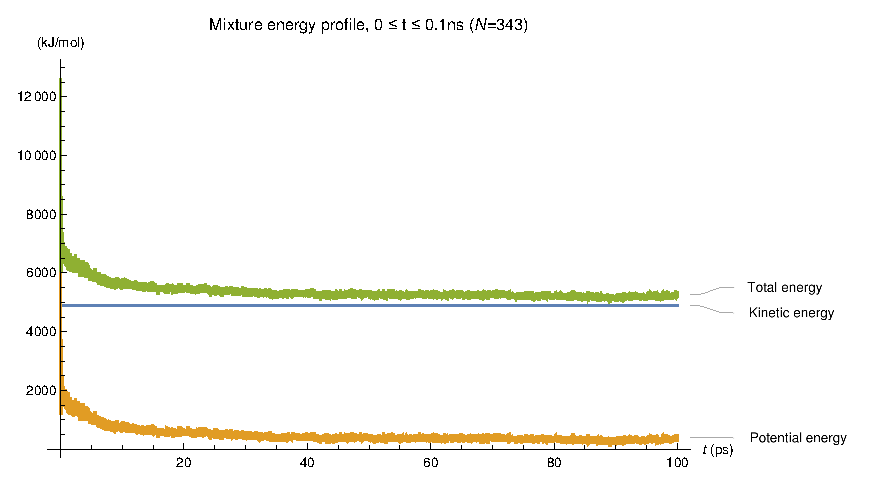
\includegraphics[scale=0.8]{figures/emix2}
\caption{Energy profile of 13.5\% mixture simulation at 300K - first steps}\label{fig:emix2}
\end{figure}

\begin{figure}
\centering
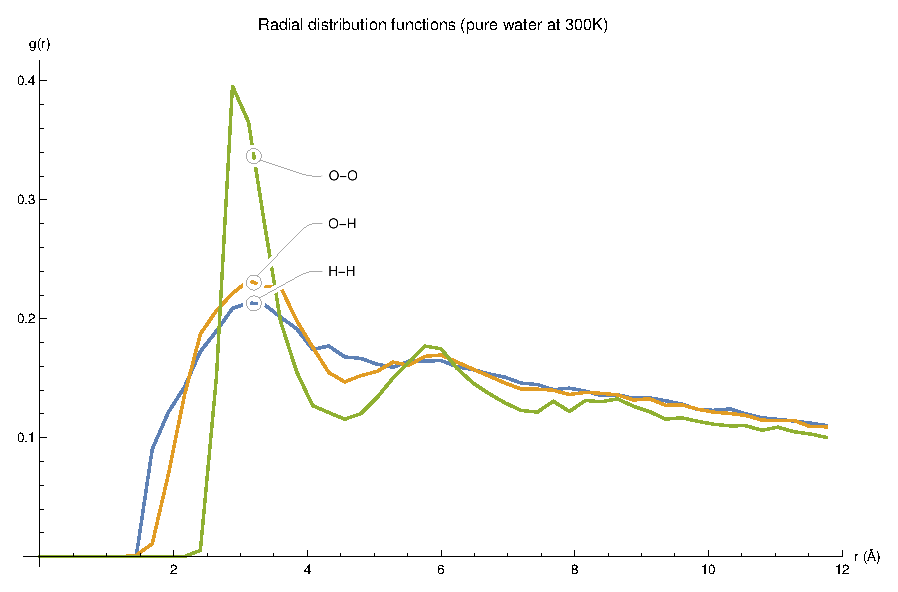
\includegraphics[scale=0.8]{figures/rdfwater}
\caption{Estimated radial distribution functions for all hydrogen-hydrogen, oxygen-hydrogen and oxygen-oxygen pairs in 1000 water molecules at 300K.}\label{fig:rdfwater}
\end{figure}

\begin{figure}
\centering
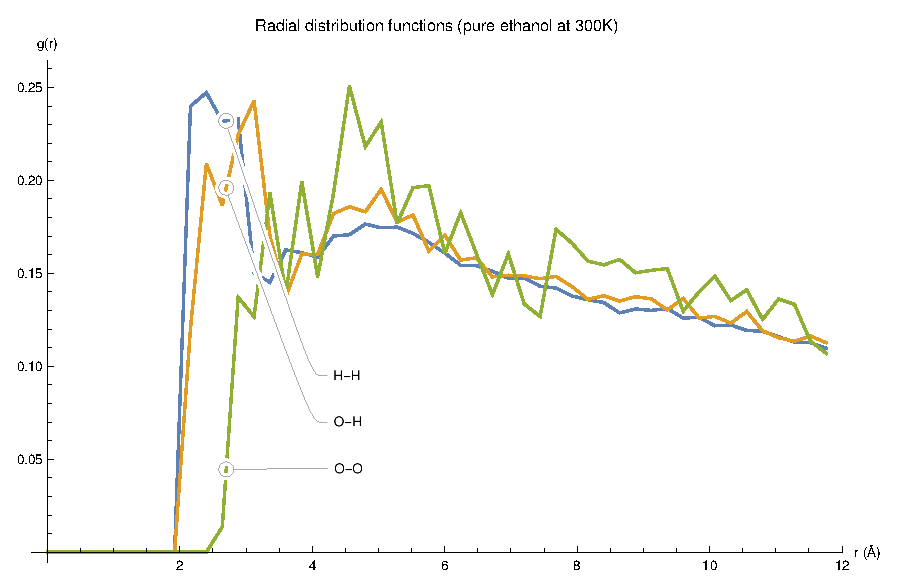
\includegraphics[scale=0.8]{figures/rdfethanol}
\caption{Estimated radial distribution functions for all hydrogen-hydrogen, oxygen-hydrogen and oxygen-oxygen pairs in 216 ethanol molecules at 300K.}\label{fig:rdfethanol}
\end{figure}

\begin{figure}
\centering
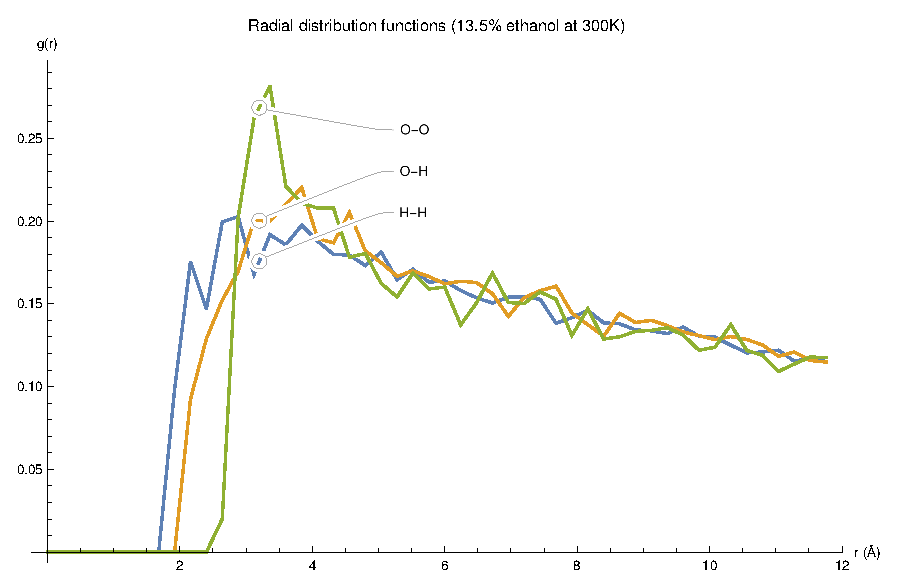
\includegraphics[scale=0.8]{figures/rdfmix}
\caption{Estimated radial distribution functions for all hydrogen-hydrogen, oxygen-hydrogen and oxygen-oxygen pairs in the 13.5\% ethanol/water mixture, with total 434 molecules at 300K.}\label{fig:rdfmix}
\end{figure}

\clearpage
\section{Notation}\label{notation}
We define the following notation and definitions:
\begin{align*}
& N & & & \textrm{The number of atoms in the system} \\
& m_i & & & \textrm{The mass of atom } i \\
& \textbf{q}_i \in \mathbb{R}^3 & & & \textrm{The position of atom } i \\
& \textbf{v}_i = \textrm{$\dot{\textbf{q}}$}_i \in \mathbb{R}^3 & & & \textrm{The velocity of atom } i \\
& \textbf{p}_i = m_i \cdot \textbf{v}_i \in \mathbb{R}^3 & & & \textrm{The momentum of atom } i \\
& \textbf{a}_i = \textrm{$\ddot{\textbf{q}}$}_i \in \mathbb{R}^3 & & & \textrm{The acceleration of atom } i \\
& T \in \mathbb{R} & & & \textrm{The temperature} \\
& k_B \approx 1.38064852\cdot 10^{-23} \; J \; K^{-1} & & & \textrm{The Boltzmann constant}
\end{align*}
Many of these quantities can vary over time. In case we would like to stress that, we can write for instance $\textbf{q}_i(t)$, $\textbf{v}_i(t)$, $\textbf{p}_i(t)$, $\textbf{a}_i(t)$ and $T(t)$. 

\section{Code}
\label{code}

\subsection{Simulation.py}
	\lstinputlisting[language=Python]{code/SimulationForLatex.py}
\clearpage

\subsection{functionsSimulation.py}
	\lstinputlisting[language=Python]{code/functionsSimulationForLatex.py}
\clearpage

\subsection{radials.py}
	\lstinputlisting[language=Python]{code/radials.py}

\end{document}